% file: cheatsheet_cs.tex
\documentclass[11pt,a4paper]{article}

% ------------------ Math ------------------
\usepackage{amsmath, amssymb, amsthm}

% ------------------ Page layout ------------------
\usepackage{geometry}
\geometry{margin=2.5cm}

% ------------------ Hyperlinks ------------------
\usepackage{hyperref}
\hypersetup{colorlinks=true, linkcolor=blue, urlcolor=blue}

% ------------------ Titles ------------------
\usepackage{titlesec}
\titleformat{\section}
  {\normalfont\Large\bfseries\centering}  
  {\thesection}{1em}{}

% ------------------ Header and footer ------------------
\usepackage{fancyhdr}
\pagestyle{fancy}
\fancyhead{} % clear all headers
\fancyfoot{} % clear all footers
\fancyhead[L]{Gabriele Perna}          
\fancyhead[C]{Must Know}     
\fancyhead[R]{2025/2026}             
\fancyfoot[C]{\thepage}           

% ------------------ Graphics ------------------
\usepackage{graphicx}    % include images
\usepackage{tikz}        % diagrams
\usetikzlibrary{trees,shapes,arrows.meta,positioning}
\usepackage{pgfplots}    % plotting graphs
\pgfplotsset{compat=1.18}

% ------------------ Tables ------------------
\usepackage{longtable}
\usepackage{booktabs}
\usepackage{multicol}

% ------------------ Floats and captions ------------------
\usepackage{caption}
\usepackage{float}

% ------------------ Code listings ------------------
\usepackage{listings}

% ------------------ Document info ------------------
\title{Must Know per Studenti di Informatica}
\author{Raccolta: concetti fondamentali}

% Automatically start each section on a new page
\let\oldsection\section
\renewcommand{\section}{\clearpage\oldsection}

\begin{document}

\maketitle
\tableofcontents
\bigskip

% ------------------ Document content starts here ------------------


\section{Matematica di base}

\subsection{Formula di Gauss (somma dei primi \(n\) naturali)}
La formula di Gauss per la somma dei primi \(n\) numeri naturali è:
\[
\sum_{k=1}^n k = 1 + 2 + \dots + n = \frac{n(n+1)}{2}.
\]
\textbf{Dimostrazione rapida (argomento classico):} Disponi la somma in ordine crescente e decrescente:
\[
S = 1 + 2 + \dots + n,
\qquad
S = n + (n-1) + \dots + 1.
\]
Sommandole membro a membro otteniamo \(2S = n(n+1)\), quindi \(S = \dfrac{n(n+1)}{2}\).

\paragraph{Esempio:} per \(n=100\), la somma è \(\dfrac{100\cdot 101}{2} = 5050\).

\subsection{Successione di Fibonacci e Formula di Binet}
La successione di Fibonacci è definita ricorsivamente:
\[
F_0 = 0,\quad F_1 = 1,\quad F_{n} = F_{n-1} + F_{n-2}\quad (n\ge 2).
\]
\textbf{Formula chiusa (Binet):}
\[
F_n = \frac{\varphi^n - \psi^n}{\varphi - \psi}
\quad\text{dove}\quad
\varphi = \frac{1+\sqrt{5}}{2},\quad \psi = \frac{1-\sqrt{5}}{2}.
\]
Poiché \(|\psi|<1\), per \(n\) grande \(F_n\) è molto vicino a \(\varphi^n/\sqrt{5}\).

\paragraph{Derivazione (breve):} Risolvi l'equazione caratteristica \(r^2 = r + 1\), ottieni le radici \(\varphi\) e \(\psi\), quindi esprimi la soluzione della ricorrenza come combinazione lineare \(A\varphi^n + B\psi^n\) e usa condizioni iniziali per determinare \(A\) e \(B\).

\subsection{Congettura di Collatz}
La congettura di Collatz (o 3\(n\)+1) è una domanda aperta semplice da enunciare:
\begin{itemize}
  \item Definisci la funzione \(T:\mathbb{N}\to\mathbb{N}\) così:
  \[
  T(n)=\begin{cases}
  n/2 & \text{se } n \text{ è pari}\\
  3n+1 & \text{se } n \text{ è dispari.}
  \end{cases}
  \]
  \item Partendo da qualsiasi \(n\in\mathbb{N}\), iterando \(T\) si ottiene una sequenza. La congettura afferma che per ogni \(n\) la sequenza raggiunge 1.
\end{itemize}
La congettura non è dimostrata né confutata in generale, ma è stata verificata per moltissimi valori numerici con calcolatori.

\section{Sistemi di numerazione e alfabeti}
\subsection{Alfabeto greco (frequente in matematica e informatica)}
\begin{figure}[h]
    \centering
    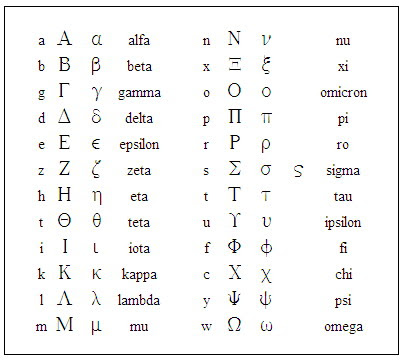
\includegraphics[width=0.9\textwidth]{images/GreekAlphabet.jpg} % replace with your file name
    \caption{Alfabeto greco}
    \label{fig:greek}
\end{figure}
Nota: alcune lettere hanno varianti grafiche usate in contesti diversi (es. \(\epsilon\) vs \(\varepsilon\), \(\phi\) vs \(\varphi\), \(\sigma\) vs \(\varsigma\)).

\subsection{Numeri romani}
\begin{center}
\begin{tabular}{ll}
\toprule
Simbolo & Valore \\
\midrule
I & 1 \\
V & 5 \\
X & 10 \\
L & 50 \\
C & 100 \\
D & 500 \\
M & 1000 \\
\bottomrule
\end{tabular}
\end{center}
Esempi: IV = 4, IX = 9, XL = 40, XC = 90.

\subsection{Alfabeto esadecimale (hex)}
L'esadecimale usa cifre 0--9 e lettere A--F per rappresentare valori 0--15:
\[
\{0,1,2,3,4,5,6,7,8,9,A,B,C,D,E,F\}.
\]
Esempio: \texttt{0x1A3F} rappresenta \(1\cdot 16^3 + 10\cdot 16^2 + 3\cdot 16 + 15\).


\section{Programmazione e pratica}

\subsection{Pseudocodice per Fibonacci (iterativo vs ricorsivo)}
\paragraph{Ricorsivo (leggibile ma inefficiente):}
\begin{lstlisting}[language=,basicstyle=\small\ttfamily]
function fib(n):
    if n == 0: return 0
    if n == 1: return 1
    return fib(n-1) + fib(n-2)
\end{lstlisting}
La versione ricorsiva ha complessità esponenziale \(O(\varphi^n)\) senza memoization.

\paragraph{Iterativo/dinamico (efficiente):}
\begin{lstlisting}[language=,basicstyle=\small\ttfamily]
function fib_iter(n):
    a = 0; b = 1
    for i = 2 to n:
        tmp = a + b
        a = b
        b = tmp
    return b  # O(n) tempo, O(1) spazio
\end{lstlisting}

\end{document}
